\section{Gas: drift velocity and attachment}\label{sec:gas}
\sectionstate{partial}{\texttt{sps\_beam\_test\_26/analysis/cloud\_basics} \S16--27 (FINDINGS); notes \texttt{mx17-beam-attachment}, \texttt{mx17-sps-to-bench}}
\intent{The gas the chambers actually ran with, measured from the waveforms with one physics model and no free
loss rate: water sets the drift velocity, O$_2$ sets the attachment.}

\tbw{Bench (det3 drift scan, six fields 35--382\,V/cm): $v$ = 2.5--37.8\,\textmu m/ns, 0.95\,\% water, no air
($\lesssim$10\,ppm O$_2$). Beam run\_71: 1.51\,\% water and 163\,ppm O$_2$, attachment measured in X and Y;
run\_63 230$\to$147\,ppm overnight. The beam O$_2$ does not spoil the SPS readout constants. Gap topography
(bench det3 spread 1.5\,mm). Magboltz~\cite{Biagi1999}.}
\analysis{D2}{v(E) points reconstructed on r06}
\analysis{D5}{three-body O$_2$ attachment scale (ppm is model-dependent)}
\askStephan{Gas system on the bench: flow, materials, expected outgassing / water ingress?}

\begin{figure}[t]
  \centering
  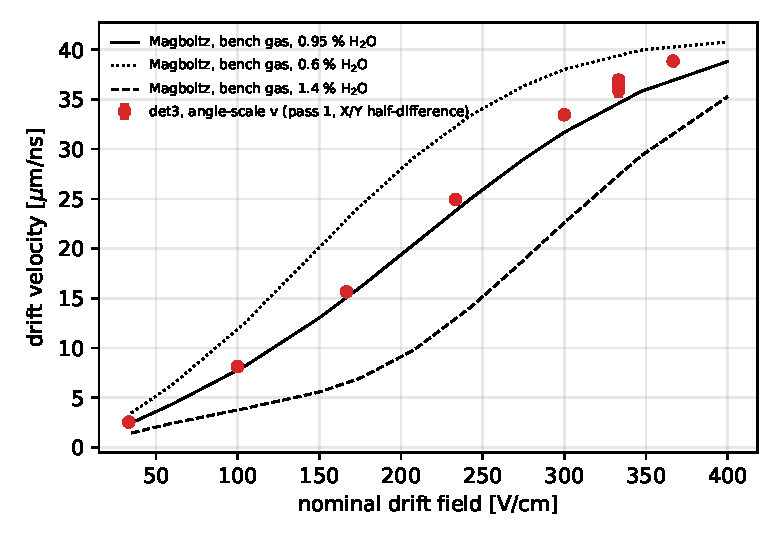
\includegraphics[width=0.7\linewidth]{gas_vE}
  \caption{\tbw{Drift velocity against field, waveform fit and Magboltz.}}
  \label{fig:vE}
\end{figure}
\begin{figure}[t]
  \centering
  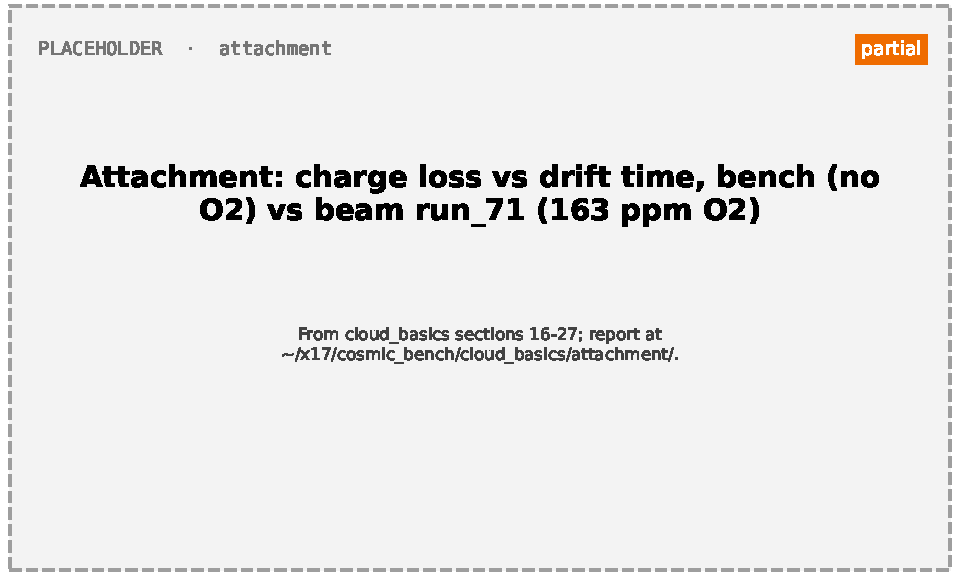
\includegraphics[width=0.7\linewidth]{attachment}
  \caption{\tbw{Charge loss with drift time: bench and beam.}}
  \label{fig:attach}
\end{figure}
